\documentclass{article}

\usepackage{graphicx}
\usepackage{tikz}
\usepackage{tikzsymbols}
\usetikzlibrary{calc,patterns,shapes.geometric}
\pagestyle{empty}
\usepackage[margin=0pt]{geometry}
\geometry{papersize={14in,12in}}

\def\centerarc[#1](#2)(#3:#4:#5){\draw[#1] ($(#2)+({#5*cos(#3)},{#5*sin(#3)})$) arc (#3:#4:#5);}

\begin{document}
	\begin{figure}
		\centering
		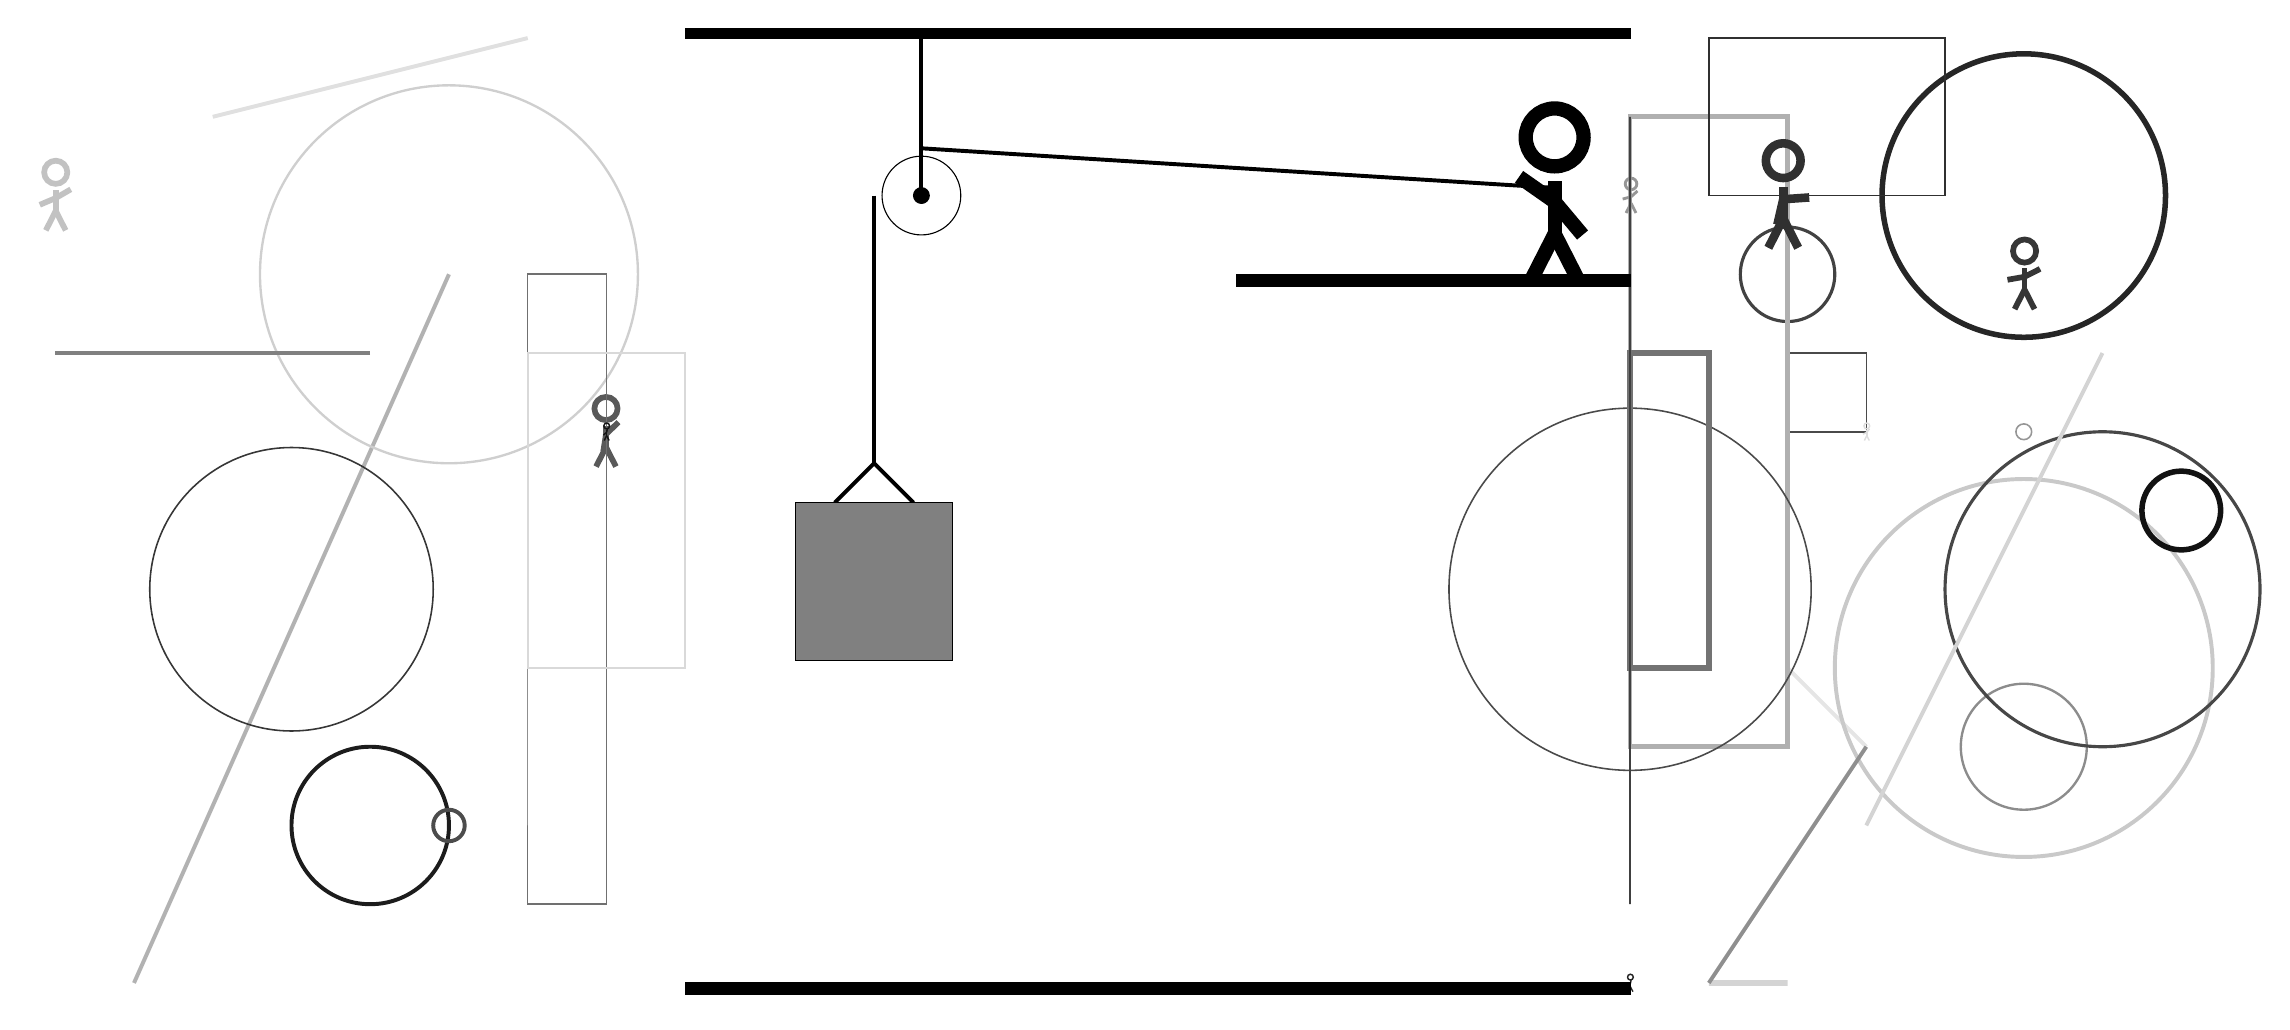
\begin{tikzpicture}
			%%%%% START %%%%%
			
			\draw[fill=black] (-2, 9) rectangle (10, 9.125);
			
			\draw (1, 7) circle (0.5);
			\draw[fill=black] (1, 7) circle (0.1);
			\draw[line width=0.5mm] (1, 9) -- (1, 7);
			
			\draw[line width=0.5mm](-0.1, 3.1) --  (0.4, 3.6) -- (0.9, 3.1);
			\draw[fill=black!50] (-0.6, 3.1) rectangle (1.4, 1.1);
			
			\node[line width=0.2mm, color=black!86] at (10, -3) {\Strichmaxerl[1][34][80]};
			
			\draw[line width=0.5mm, color=black!10](12, 1) -- (13, 0);
			\draw [line width=0.4mm, color=black!74](12, 6) circle (0.6);
			\draw[line width=0.7mm, color=black!17] (12, -3) rectangle (11, -3);
			
			\draw[line width=0.2mm, color=black!71] (12, 5) rectangle (13, 4);
			
			\draw [line width=0.3mm, color=black!45](15, 0) circle (0.8);
			\node[line width=0.5mm, color=black!65] at (-3, 4) {\Strichmaxerl[4][81][44]};
			\draw[line width=0.5mm, color=black!30](-5, 6) -- (-9, -3);
			\draw [line width=0.7mm, color=black!85](15, 7) circle (1.8);
			\draw[line width=0.6mm, color=black!31] (10, 8) rectangle (12, 0);
			\draw [line width=0.5mm, color=black!21](15, 1) circle (2.4);
			
			\draw [line width=0.3mm, color=black!19](-5, 6) circle (2.4);
			\draw[line width=0.5mm, color=black!44](13, 0) -- (11, -3);
			
			\draw[line width=0.2mm, color=black!56] (-3, 6) rectangle (-4, -2);
			\draw [line width=0.5mm, color=black!89](-6, -1) circle (1.0);
			\draw [line width=0.5mm, color=black!70](-5, -1) circle (0.2);
			\node[line width=0.4mm, color=black!41] at (10, 7) {\Strichmaxerl[2][15][42]};
			
			\draw [line width=0.2mm, color=black!71](10, 2) circle (2.3);
			\draw [line width=0.4mm, color=black!72](16, 2) circle (2.0);
			
			\node[line width=0.3mm, color=black!79] at (15, 6) {\Strichmaxerl[4][10][27]};
			\draw[line width=0.2mm, color=black!81] (11, 9) rectangle (14, 7);
			
			\node[line width=0.6mm, color=black!13] at (13, 4) {\Strichmaxerl[1][25][52]};
			\draw[line width=0.2mm, color=black!44] (-4, -1) rectangle (-4, 1);
			\draw [line width=0.7mm, color=black!93](17, 3) circle (0.5);
			\draw[line width=0.7mm, color=black!55] (10, 1) rectangle (11, 5);
			
			\node[line width=0.7mm, color=black!24] at (-10, 7) {\Strichmaxerl[4][23][30]};
			\draw[line width=0.3mm, color=black!11] (10, 0) rectangle (10, 2);
			\draw[line width=0.3mm, color=black!15] (-2, 1) rectangle (-4, 5);
			\node[line width=0.4mm, color=black!81] at (12, 7) {\Strichmaxerl[6][77][4]};
			\draw [line width=0.2mm, color=black!79](-7, 2) circle (1.8);
			\node[line width=0.4mm, color=black!92] at (-3, 4) {\Strichmaxerl[1][39][80]};
			
			\draw[line width=0.5mm, color=black!50](-6, 5) -- (-10, 5);
			\draw[line width=0.5mm, color=black!17](13, -1) -- (16, 5);
			\draw [line width=0.2mm, color=black!41](15, 4) circle (0.1);
			\draw[line width=0.5mm, color=black!12](-4, 9) -- (-8, 8);
			\draw[line width=0.3mm, color=black!75] (10, -2) rectangle (10, 8);
			
			\draw[line width=0.5mm](0.4, 7) -- (0.4, 3.6);
			\centerarc[line width=0.5mm](1, 7)(90:180:0.6)
			\draw[line width=0.5mm](1, 7.6) -- (9, 7.1);
			
			\node at (9, 7) {\Strichmaxerl[10][-35][-50]};
			\draw[fill=black] (5, 6) rectangle (10, 5.85);
			
			\draw[fill=black] (-2, -3) rectangle (10, -3.15);
			
			%%%%% END %%%%%
		\end{tikzpicture}
	\end{figure}	
\end{document}